\section{势能损失函数}
如上节所述,我们把模型补全攻击考虑为攻击者基于泄露数据的机器学习过程。
%
本节我们研究攻击者在泄露样本上学习得到的顶部模型的泛化误差。
我们通过二分类例子表明当拆分层表征分布在决策边界附近时,攻击者的泛化误差较大。
同时,数据分布在决策边界时,类间距离减小,类内距离加大,因此聚类攻击的效果也下降。
%
受到静电平衡理论以及库仑定律的启发,我们提出了势能损失,使得拆分层表征满足上述的分布,从而实现对于模型补全攻击的保护。
%

\subsection{数据分布导致的学习误差}
我们从微调攻击的泛化误差以及聚类误差两个角度来说明同类样本分布在决策边界附近时可以使得攻击者的学习误差变大。


\subsubsection{泛化误差}
直观地说,当同类表征分布在决策边界附近时,表明同类表征之间的距离加大,从而使得少量该类别的表征无法代表整个类别的表征,因此会提高攻击者在少量样本上训练顶部模型的泛化误差。
%
下面我们使用一个二分类的例子对其进行说明。
%

考虑表征空间为一个$d$维超球体($d$-sphere)$\{ \bvec{x}: \sum_{i=1}^d h_i^2 = 1\}$,所有表征被划分为两个类别(正样本和负样本)。
令假设集(Hypothesis Set, 即所有可能的分类函数的集合)为所有的半球面(表示正样本)集合:
\begin{equation}
    \mathcal H = \{ h: h(\bvec{x}) = \text{Sign}(\bvec{w} \cdot \bvec{x}), \Vert \bvec{w} \Vert_2 = 1\}.
\end{equation}
不失一般性,我们假设目标分类函数为$f(\bvec{x}) = \text{Sign}(x_1)$。
同时,我们对表征的分布做出如下假设:
\begin{itemize}
    \item 表征分布的概率密度仅仅和其坐标的第一维有关,也就是仅和$x_1$有关,而在其他维度上呈现出各向同性(Isotropic)性质。
    \item 给定一批正样本数据$S = \{\bvec{x}_1, \cdots, \bvec{x}_n\}$,学习算法简单地产生其归一化(Normalized)的平均值作为学到的分类模型的权重$\bvec{w}$。
    即:
    \begin{equation}
        f^{(S)}(\bvec{x}) = \text{Sign}\left[ \bvec{x} \cdot \sum_{i=1}^n {\bvec{x}_i} / \Vert \sum_{i=1}^n {\bvec{x}_i}\Vert_2 \right].
    \end{equation}
\end{itemize}

考虑当学习到的参数$\bvec{w} = \sum_{i=1}^n \bvec{x}_i / \Vert \sum_{i=1}^n \bvec{x}_i \Vert_2$ 与目标分类模型的参数 $\bvec{e}_1$ 有一点偏差时的情况。
%
由于我们假设表征的分布在$\bvec{e}_1$之外的维度时各向同性的,我们可以假设$\bvec{w}$位于前两维展开的超平面上,也就是
\begin{equation}
    \bvec{w} = \bvec{e}_1 \cos \epsilon + \bvec{e}_2 \sin \epsilon,    
\end{equation}
其中$\epsilon$表示$\bvec{w}$和$\bvec{e}_1$之间的一个小角度。
%
此时我们可以得到泛化误差为:
\begin{equation}
\begin{split}
    1/2\cdot R[\bvec{w}] &= \mathop{\mathbb E}_{\bvec{x} \sim \mathcal S} \text{Sign}(x_1) \cdot I[x_1 \cos \epsilon + x_2 \sin \epsilon \le 0]
    \\
    & = \int_{\substack{x_1 > 0 \\ x_1 \cos \epsilon + x_2 \sin \epsilon \le 0 \\ x_1^2 + \cdots + x_d^2 = 1}} p(x_1, \cdots, x_d)dS
      \le \int_{\substack{x_1^2 + ... + x_d^2 = 1 \\0 < x_1 \le \tan\epsilon}}p(x_1, x_2, ...,x_d)dS
\end{split}
\end{equation}
注意到当$\epsilon \to 0$时,$\tan \epsilon \to \epsilon$,并且令$p_1$为表征在$\bvec{e}_1$上的边缘概率密度,即$p_1(x_1) = \int_{x_1^2 + \cdots + x_d^2} p(x_1, \cdots, x_d) dx_2\cdots dx_d$,
%
上式右侧可以进一步化为
\begin{equation}
    \int_{\substack{x_1^2 + ... + x_d^2 = 1 \\0 < x_1 \le \tan\epsilon}}p(x_1, x_2, ...,x_d)dS \approx \int_{x_1 = 0}^{\epsilon} p_1(x_1) dx_1 \approx \epsilon p_1(0).
\end{equation}
%
从上式可以看出,当$\epsilon$很小时,泛化误差的上界与$p_1(0)$呈近似线性关系。
因为$p_1(0)$就是正样本和负样本交界处的表征边缘概率密度,所以也可以说,此时泛化误差的大小与表征在决策边界附近的概率密度时成比例的。
越多的表征分布在决策边界上,则分类函数的误差导致的泛化误差就越大。

在上面的讨论中,我们假设$\epsilon$是一个固定的小量。
%
现在我们来讨论$\epsilon$与表征分布的关系。
%
对于任何一个随机变量$X$,如果$X_1, \cdots, X_m$是$m$个独立的采样,则有:
\begin{equation}
    \mathbb E \left[ \left(\dfrac{1}{m}\sum_{i=1}^m h_i - \mathbb E[X] \right)^2 \right] = \dfrac{1}{m} \mathbb E\left[\left(X -\mathbb EX\right)^2 \right].
\end{equation}
%
也就是说,如果随机变量的分布远离其均值,则多次采样后得到的采样均值相对于实际分布的均值的误差就越大。
%
虽然在先前的讨论中,我们假定表征空间是一个超球面,但是上述结论依然是近似成立的,也就是 $\mathbb E[\epsilon^2]\propto \mathbb E\left[(X - \mathbb EX)^2\right]$。
为了使得决策区域误差 $\epsilon$ 尽可能变大,同一类别的表征应该尽量分布在远离其分布均值的区域。
同时我们也可以注意到,离某一类别表征分布均值最远的区域也正是该类别的决策边界。
%
已有的从数据分布直接推导泛化误差上界的研究与上文的分析较为类似~\cite{jinpengzhan2020generalization},该研究使用数据的类内距离和类间距离对泛化误差上界进行估计。


%
\subsubsection{聚类误差}
当表征分布于决策边界附近时,对其进行聚类也将变得困难。
%
因为聚类的基本思想是把距离较近的一群数据点归入一个簇中,也就是说,聚类之后的每个类别里面的数据点应该彼此靠近~\cite{saxena2017cluster_review}。
%
但是通过让表征分布到决策边界上,与其分布均值远离,同类表征之间的距离变得更大了,而不同类表征之间的距离变得更小了。
%
这便与聚类的基本要求相违背,因此让表征分布于决策边界的做法很显然可以降低对其聚类的效果。


\subsubsection{总结}
综上所述,让表征分布到自身类别的决策边界,可以同时提高对其进行微调或聚类的学习误差,其原因可以总结为以下三点:
\begin{itemize}
    \item 学习得到的决策区域的误差$\epsilon$变大。
    \item 同样的决策区域误差$\epsilon$导致的模型泛化误差变大。
    \item 类间距离变小,类内距离变大。
\end{itemize}
我们将上述的分析直观地在\autoref{fig:peloss:method}中显示。

\begin{figure}[h!]
    \centering
    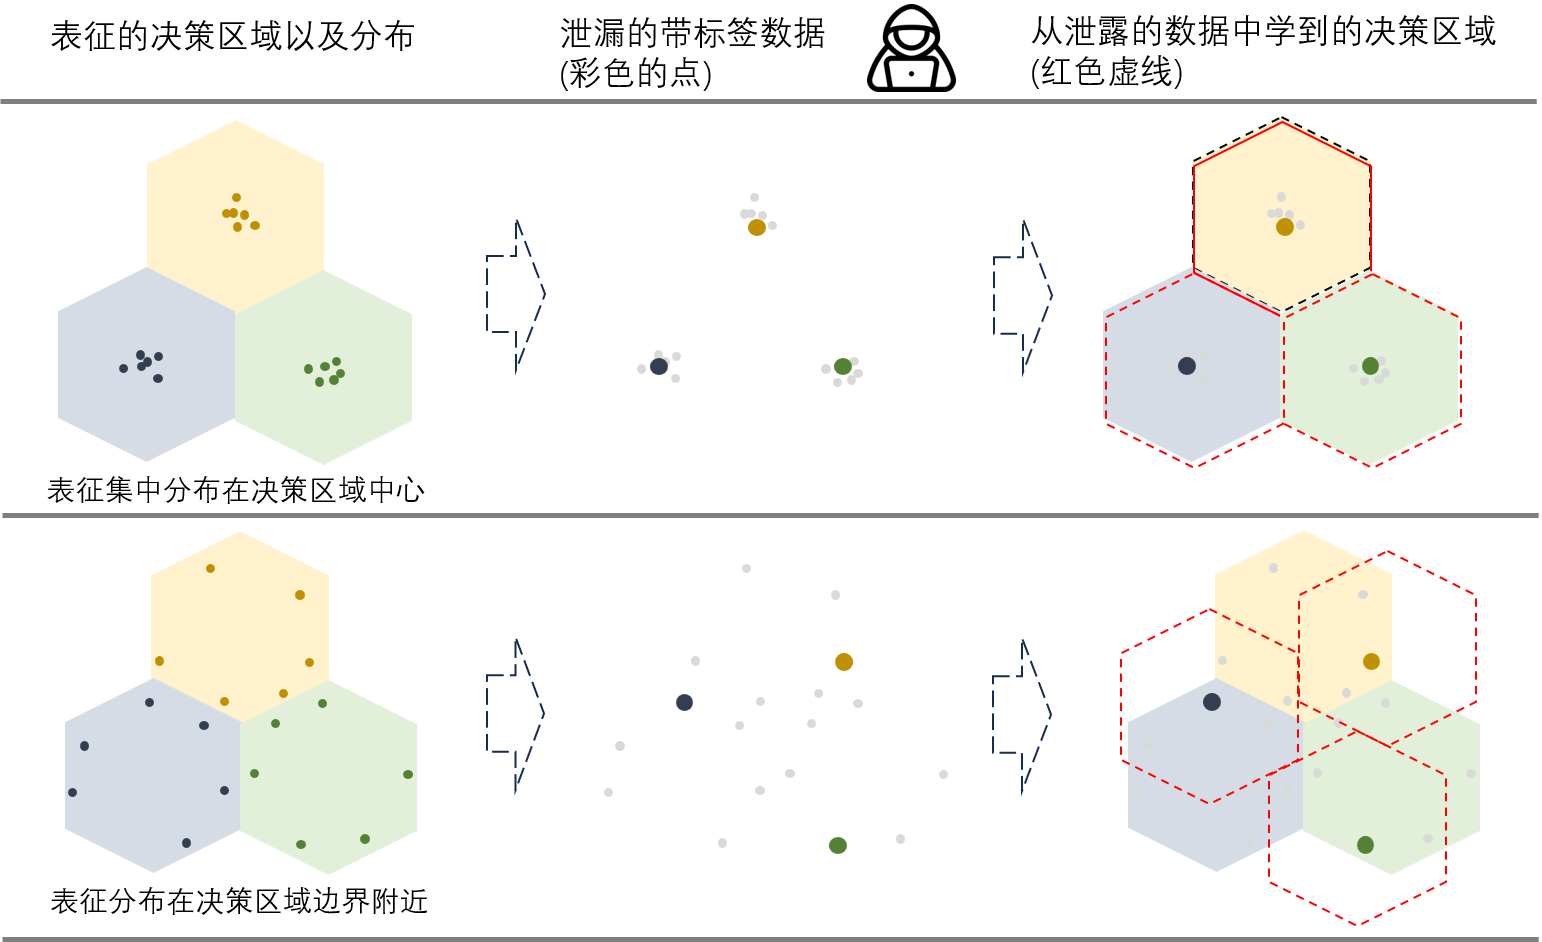
\includegraphics[width=1\linewidth]{Z_Resources/peloss_method.png}
    \caption{隐层表征分布导致的攻击者误差示意图}
    \label{fig:peloss:method}
\end{figure}


\subsection{势能损失函数定义}
物理学中的静电平衡(Electrost Equilibrium)现象告诉我们,当一个导体建立静电平衡时,其所有净电荷(Net Charge)将会分布在导体表面~\cite{griffiths2005introduction}。
%
这个现象的一部分原因时库仑定律(Coulomb's Law),即:同性电荷之间相互排斥,而异性电荷之间相互吸引。
%
受到该物理现象的启发,我们可以把相同类别的表征看作同性电荷,使得它们之间存在互相排斥对方的斥力。
因此,这些同类别的表征就会相互远离直到决策区域的边界处。
%

库仑定律的公式为
\begin{equation}
\label{eq:peloss:columb}
    \bvec{F} =  k {q_1q_2(\bvec{r}_1 - \bvec{r}_2)}/{\Vert r_1 - r_2 \Vert_2^3},
\end{equation}
其中,$k$表示一个常数,$q_1, q_2$时带符号的电荷大小(正电荷为正号,负电荷为负号),$\bvec{r}_1, \bvec{r}_2$表示两个电荷的位置,$\Vert \cdot \Vert$表示欧几里得范数,$\bvec{F}$则表示第二个电荷对第一个电荷产生的力(库仑力)的大小。
%
我们忽略常数以及电荷的大小,只考虑同性电荷,则可以把\autoref{eq:peloss:columb}化为$\bvec{F} = (\bvec{r}_1 - \bvec{r}_2) / \Vert\bvec{r}_1 - \bvec{r}_2 \Vert_2^3$。
%
由于库仑力也可以表示为电势能的梯度,我们可以进一步将其表示为梯度的形式$F = \nabla_{\bvec{r}_1} 1/\Vert \bvec{r}_1 - \bvec{r}_2 \Vert_2$。
%
这种表示方法与深度学习中所使用的梯度下降方法不谋而合。
%
基于以上分析,我们定义势能损失函数为:
\begin{equation}
    L_\text{pe} = \sum\limits_{c\in\mathcal C}\sum\limits_{\bvec{h} \in H_c}\sum\limits_{\bvec{h}' \in H_c, \bvec{h}' \ne \bvec{h}} \dfrac{1}{\Vert \bvec{h} - \bvec{h'} \Vert_2},
\end{equation}
其中$\mathcal C$表示标签的集合,$H_c$表示类别为$c$的表征集合。


通过把$L_{pe}$加入损失函数中,在拆分模型的训练过程中,同类别的表征互相之间会排斥并且逐渐移动到该类别的决策区域边界处。
%
在三维的情况下,汤姆森定理(Thomson's Theorem)证明电势能最小的情况对应于电荷全部分布在导体的表面,也就是表征的概率质量全部在决策边界~\cite{griffiths2005introduction}。
%
但是考虑到拆分层的表征空间的维度一般远大于3维,因此其概率质量并不能完全集中在决策边界。
但是我们依然能证明,在势能损失函数最小的情况下,决策边界处必然有概率质量分布。

\begin{theorem}[决策边界的表征分布非零]
\label{thm:peloss:border-distribution}
    考虑一个$d$维有界区域$\Omega \subset \mathbb R^d$以及定义在$\Omega$内部的概率密度泛函$f^*$为最小化势能损失的概率密度:
    \begin{equation}
        \label{eq:peloss:potential-min}
        f^* = \mathop\textnormal{argmin}_f \textnormal{PE}(f) = \mathop\textnormal{argmin}_{f} \int_{\bvec{x} \in \Omega} \int_{y \in \Omega} \dfrac{f(\bvec{x})f(\bvec{y})}{\Vert \bvec{x} - \bvec{y} \Vert_2} dUdV,
    \end{equation}
    其中,$f$表示概率密度函数且满足$f \ge 0$(非负性) 以及 $\int_{\Omega} f(\bvec{x})dV = 1$(归一性)。
    令$\Delta_\epsilon \Omega = \{\bvec{x}: \bvec{x} + \epsilon \bvec{r} \not\in \Omega, \bvec{x} \in \Omega, \Vert \bvec{r} \Vert_2 = 1 \}$ 表示距离$\Omega$边界距离小于$\epsilon$的区域,那么$f^*$满足对于任意$\epsilon > 0$,有$\int_{\bvec{x}\in\Delta_\epsilon \Omega} f^*(\bvec{x})dV > 0$。
\end{theorem}
\begin{proof}
    为了证明的方便,此处我们用$|\cdot |$来表示欧几里得范数。
    %
    首先考虑中心在$\bvec{x}_0$,半径为$r$的球$B_r(\bvec{x}_0)$。
    令
    \begin{equation}
        r_0 = \inf_r \left\{ \int_{\bvec{y}\in \Omega - B_{r}(\bvec{x}_0)} f(\bvec{y}) dV = 0 \right\},
    \end{equation}
    即:$f(x)$ 在$B_{r_0}(x_0)$ 之外几乎处处为0,也就是说$B_0 = B_{r_0}(x_0)$是以$x_0$为中心且包含了几乎所有概率质量的最小半径球。
    %
    因此我们可以找到一个靠近$B_0$边界的小球$B_1 = B_{\epsilon/4}(\bvec x_0 + \bvec{r}')$使得
    $\int_{\bvec{y}\in B_1} f(\bvec{y})dV = \delta$,其中$\delta > 0$,$|\bvec{r}'| = r_0 - \epsilon / 4$。
    也就是说,$B_1$内部的概率质量非零。
    %

    现在我们考虑将$f$在$B_1$里面的概率质量移动到$B_2 = B_{\epsilon/4}(\bvec x_0 + \bvec{r}'(1 + \dfrac{3\epsilon}{4|r'|})) = B_{\epsilon/4}(\bvec x_0 + \bvec{r}'')$中。
    %
    由于$B_2 \subset \Delta_\epsilon \Omega$且$B_1 \subset \Omega - \Delta_\epsilon \Omega$,所以上述的移动是可行的。
    %
    我们把概率质量移动后的概率密度函数记作
    \begin{equation}
        f'(\bvec{t}) = \begin{cases}
            f(\bvec{t} - \bvec{r}'' + \bvec{r}') & \quad \text{当 $\bvec{t} \in B_2$},\\
            0               & \quad \text{当 $\bvec{t} \in B_1$},\\
            f(t)            & \quad \text{其他}.
        \end{cases}
    \end{equation}
    此时我们计算$f'$和$f$的势能差异(把$\Omega - B_1 - B_2$记作$\Omega'$):
    \begin{equation}
    \label{eq:peloss:diff0}
    \small
    \begin{split}
        & \text{PE}(f) - \text{PE}(f') 
        = \int_{\bvec{x} \in \Omega} \int_{\bvec{y} \in \Omega} \dfrac{f(\bvec{x})f(\bvec{y}) - f'(\bvec{x})f'(\bvec{y})}{|\bvec{x}-\bvec{y}|}dUdV 
        \\
        & = 
        \left( 
            \int_{\bvec{x} \in B_1 \cup B_2} \int_{\bvec{y} \in \Omega'} + 
            \int_{\bvec{x} \in \Omega'} \int_{\bvec{y} \in B_1 \cup B_2} +
            \int_{\bvec{x} \in B_1 \cup B_2} \int_{\bvec{y} \in B_1 \cup B_2}
        \right) 
        \dfrac{f(\bvec x)f(\bvec y) - f'(\bvec x)f'(\bvec y)}{|\bvec x - \bvec y|}dUdV
        \\
         & = 2 \int_{\bvec x \in B_1} \int_{\bvec y \in \Omega'} \dfrac{f(\bvec x)f(\bvec y)}{|\bvec x-\bvec y|}dUd -
             2 \int_{\bvec x \in B_2} \int_{\bvec y \in \Omega'} \dfrac{f'(\bvec x)f(\bvec y)}{|\bvec x-\bvec y|}dUdV + \\
            &\quad 
            \int_{\bvec x \in B_1} \int_{\bvec y \in B_1} \dfrac{f(\bvec x)f(\bvec y)}{|\bvec x-\bvec y|}dUdV -
            \int_{\bvec x \in B_2} \int_{\bvec y \in B_2} \dfrac{f'(\bvec x)f'(\bvec y)}{|\bvec x-\bvec y|}dUdV.
    \end{split}
    \end{equation}
注意到$f'$是把$f$在$B_1$处的值直接移动到了$B_2$,因此上式最后两项可以相消。
此时可以把\autoref{eq:peloss:diff0}写成:
\begin{equation}
\label{eq:peloss:diff1}
        \dfrac{1}{2}[\text{PE}(f) - \text{PE}(f')] =
        \int_{\bvec x \in B_1} \int_{\bvec y \in \Omega'} \dfrac{f(\bvec x)f(\bvec y)}{|\bvec x- \bvec y|}dUdV
        -
        \int_{\bvec x \in B_2} \int_{\bvec y \in \Omega'} \dfrac{f'(\bvec x)f(\bvec y)}{|\bvec x- \bvec y|}dUdV.
\end{equation}
令$g(\bvec{s}) = f(\bvec{x} - \bvec{r}') = f'(\bvec{x} - \bvec{r}''), \bvec s \in B_{\epsilon/4}(0)$,则可以讲上式进一步简化为
\begin{equation}
\label{eq:peloss:diff2}
    \int_{\bvec x \in B_{\epsilon/4}(0)}\int_{\bvec y \in \Omega'} g(\bvec x)f(\bvec y) \left[ \dfrac{1}{|\bvec x + \bvec r' - \bvec y|} - \dfrac{1}{|\bvec x + \bvec r'' - \bvec y|} \right]dUdV.
\end{equation}
由于$\bvec r'$ 和 $\bvec r''$ 方向一致(我们将其对应的单位向量记作$\bvec e_r$),因此我们可以将$bvec x$和$\bvec y$分解为与$\bvec e_r$相同的方向和与其正交的方向:
\begin{equation}
    \begin{cases}
        \bvec x_r = (\bvec x \cdot \bvec e_r) \bvec e_r \\
        \bvec x_v = \bvec x - \bvec x_v
    \end{cases} 
    \quad \text{以及} \quad
    \begin{cases}
        \bvec y_r = (\bvec y \cdot \bvec e_r)\bvec e_r \\
        \bvec y_v = \bvec y - \bvec y_v
    \end{cases}
\end{equation}
于是我们有:
\begin{equation}
\begin{cases}
    |\bvec x + \bvec r' - \bvec y|^2 & = |\bvec x_r + \bvec y_r|^2 + |\bvec x_r + \bvec r' - \bvec y_r|^2 
     = |\bvec x_v + \bvec y_v|^2 + |\bvec x_r + \bvec r' - \bvec y_r|^2, \\
    |\bvec x + \bvec r'' - \bvec y|^2 & = |\bvec x_v + \bvec y_v|^2 + |\bvec x_r + \bvec r'' - \bvec y_r|^2
    = |\bvec x_r + \bvec y_r|^2 + |\bvec x_r + \bvec r'' - \bvec y_r|^2,
\end{cases}
\end{equation}
上式最后一项的左侧是相等的,因此只需考虑右侧。
我们只需考虑考虑如下两种情况:
\begin{itemize}
    \item $|\bvec x_r + \bvec r'| \ge |\bvec y_r|$: 
    同时注意到 $|\bvec r''| > |\bvec r'|$,因此$|\bvec x + \bvec r'' - \bvec y| < |\bvec x + \bvec r' - \bvec y|$。
    \item $|\bvec x_r + \bvec r'| < |\bvec y_r|$:
    因为$|\bvec y_r| < r_0$,$|\bvec x_r + \bvec r'| \ge r_0 - \epsilon / 2$,以及$|\bvec x_r + \bvec r''| > r_0 + \epsilon / 2$,因此有
    \begin{equation}
        |\bvec x_r + \bvec r'' - \bvec y_r| > \epsilon / 2 > |\bvec y_r - (\bvec x_r + \bvec r')|.
    \end{equation}
\end{itemize}
综上,当$x \in B_{\epsilon/4}(0), y \in \Omega'$时,就有
\begin{equation}
    |\bvec x + \bvec r' - \bvec y| < |\bvec x + \bvec r'' - \bvec y|,
\end{equation}
因此,
\begin{equation}
    1 / |\bvec x + \bvec r' - \bvec y| - 1 / |\bvec x + \bvec r'' - \bvec y| > 0.
\end{equation}
带入\autoref{eq:peloss:diff2},可以得到$\text{PE}(f') < \text{PE}(f)$。
至此\autoref{thm:peloss:border-distribution}得到证明。
\end{proof}

\autoref{thm:peloss:border-distribution}表明,当势能损失最小时,表征在决策边界上的分布必然不为0,否则我们便可以通过移动一小部分的概率质量到边界处使得势能损失更小,与势能损失最小的前提相矛盾。

\textbf{加入层归一化}:
势能损失方法有一个隐含条件:某一类别的表征的决策区域需要是有界的,并且要与其他类别的表征决策区域相邻。
否则,势能损失可以把同类表征推向无穷远处或是与其他类别决策区域不相邻的“边界”,使得其保护能力降低。
%
这要求表征空间是一个有界(Bounded)并且无边界(Borderless)的流形。
%
我们简单地通过层归一化(Layer Normalization)来实现该要求。
%
经过层归一化后,拆分层的表征被投影到$d$维超球体上。
%
为了保持一致性,我们也需要改变其距离的计算方式,将欧氏距离(Euclidean Distance)转化为超球面上的测地距离(Geodesic Distance),此时势能损失函数被修改为:
\begin{equation}
    L_\text{pe} = \sum\limits_{c\in\mathcal C}\sum\limits_{\bvec{h} \in H_c}\sum\limits_{\bvec{h}' \in H_c, \bvec{h}' \ne \bvec{h}} \dfrac{1}{\arccos \langle \bvec{h}, \bvec{h'} \rangle}.
\end{equation}

最终,在模型的训练过程中,我们把势能损失加入到原有的损失函数(如交叉熵分类损失)中,并设置权重为$\alpha$。
总的损失函数为$L' = L + \alpha L_{pe}$。

\subsection{与距离相关性的关系}
已有研究采用了距离相关性将拆分层表征对输入特征~\cite{vepakomma2020nopeek}或预测标签~\cite{sunjiankai2022forward_embedding_protect}进行解耦,从而实现中拆分学习中保护数据输入特征或标签的目的。
%
我们在这里讨论对标签进行保护的情况,此时距离相关性损失可以表示为
\begin{equation}
\label{eq:peloss:dcorloss}
    L_\text{dcor} = \sum_{i=1}^n d_{i,j} d'_{i, j} \Big/ \sqrt{\sum_{i,j=1}^n d_{i, j}^2 \sum_{i,j=1}^n {d'}_{i, j}^2},
\end{equation}
%
其中,$d_{i,j}$表示样本$i$和样本$j$的表征之间的双中心(Doubly-Centered)距离,即:
\begin{equation}
    d_{i, j} = \Vert \bvec h_i - \bvec h_j \Vert_2 - \mathop{\mathbb E}_{\bvec h'\in H}\Vert \bvec h_i - \bvec h' \Vert_2 - \mathop{\mathbb E}_{\bvec h'\in H}\Vert \bvec h' - \bvec h_j \Vert_2 + \mathop{\mathbb E}_{\bvec h', \bvec h'' \in H}\Vert \bvec h' - \bvec h'' \Vert_2.
\end{equation}

类似地,$d'_{i,j}$则是样本$i$和样本$j$的标签的双中心距离,以独热(One-Hot)标签为例,则$d_{i,i} = 0, d_{i,j\ne i} = \sqrt 2$。
将其带入\autoref{eq:peloss:dcorloss},提取出其分母,得到
\begin{equation}
    \sum_{\substack{c,c'\in \mathcal C \\ c\ne c'}} \sum_{\substack{\bvec h\in H_c \\ \bvec h' \in H_c'}} \sqrt2 
    \left( 
        \Vert \bvec h - \bvec h'\Vert_2 - \overline{\Vert \bvec h - \cdot \Vert_2} - \overline{\Vert \bvec \cdot - \bvec h' \Vert_2} + \overline{\Vert \cdot - \cdot\Vert_2}, 
    \right)
\end{equation}
其中,我们用 $\overline{\Vert \bvec h - \cdot \Vert}$ 表示 $\mathbb E_{\bvec h'\in H} \Vert \bvec h - \bvec h'\Vert_2$,$\overline{\Vert \cdot - \cdot \Vert}$ 表示 $\mathbb E_{\bvec h, \bvec h'\in H} \Vert \bvec h - \bvec h'\Vert_2$,$H$表示当前批样本表征集合,$H_c$表示当前批样本中类别为$c$的表征集合。
%
可以看出最小化距离相关性损失类似于最小化表征的类间距离,而本文提出的势能损失则旨在最大化类内距离,两者之间有一定的相似性。
%
然而直观地来讲,不同类别的决策边界分布在不同的方向上,导致距离相关性的计算有更高的误差且难以优化。
%
\autoref{}中的实验结果也表明势能损失相比于距离相关性更加优越。


\subsection{输入特征的隐私保护}
尽管势能损失并未直接保护输入特征的隐私,但是间接地对其进行了保护。
%
这是因为在拆分学习中,可以通过拆分层的选择来调节输入特征和标签的隐私泄露程度。
具体而言,拆分层靠近模型输入,则输入特征隐私泄露加大;而拆分层靠近模型输出,则输出特征隐私泄露加大~\cite{abuadbba2020can_split}。
%
而通过势能损失函数,我们可以将拆分层设置到更靠近输出的位置,此时特征的隐私泄露自然也就减少了。
%
对于类似卷积神经网络的模型,其中间层会保留大量的输入数据的信息,因此通过势能损失,把拆分层设置为最后一层,可以极大提高对于输入特征的保护,
同时也保护标签的隐私。
%